\RequirePackage[l2tabu,orthodox]{nag}


%\documentclass[headsepline,footsepline,footinclude=false,fontsize=11pt,paper=a4,listof=totoc,bibliography=totoc,BCOR=12mm,DIV=12]{scrbook} % two-sided
\documentclass[headsepline,footsepline,footinclude=false,oneside,fontsize=11pt,paper=a4,listof=totoc,bibliography=totoc]{scrbook} % one-sided


\usepackage[utf8x]{inputenc}
\usepackage[ngerman]{babel}
\usepackage{graphicx}
\usepackage{lmodern}
\usepackage{hyperref}

\hypersetup{
	colorlinks =truerue,
	linktoc =all,
	linkcolor=red,
}

%Präambel
\title{Titel}
\author{Name}
\date{\today, Ort}

% Textual Commands:
\newcommand{\term}[1]{\textit{#1}}


% Default (not implemented yet function)
\newcommand{\error}{\textbf{ERROR}}


% Quotations:
\newcommand{\quot}[2]{''#1'' \cite{#2}}
\newcommand{\takenFrom}[1]{\cite[taken from][]{#1}}


% References:
\newcommand{\refFigure}[1]{\hyperref[#1]{Figure \ref{#1}}}
\newcommand{\refTable}[1]{\hyperref[#1]{Table \ref{#1}}}
\newcommand{\refChapter}[1]{\hyperref[#1]{chapter \ref{#1}}}


% Pictures:
\newcommand{\pic}{Insert Picture here \error}


% Tables:


% Math commands
\newcommand{\set}[1]{\mathcal{#1}}
\renewcommand{\vec}[1]{\bm{#1}}
\newcommand{\mat}[1]{\bm{#1}}
\newcommand{\R}{\mathbb{R}}
\newcommand{\N}{\mathbb{N}}
\newcommand{\norm}[1]{\left\|#1\right\|}
\newcommand{\trans}{{\raisebox{.1ex}{$\mathrm{\mathsmaller T}$}}}
\newcommand{\inv}{{\raisebox{.2ex}{$\mathsmaller{\text{-}1}$}}}
\newcommand{\given}{;\,}
\newcommand{\abs}[1]{\left|#1\right|}

\newcommand{\lmin}{\ell_{\text{min}}}
\newcommand{\lmint}{\ell_{\text{min}, t}}
\newcommand{\lmax}{\ell_{\text{max}}}
\newcommand{\tol}{\epsilon_{\text{tol}}}
\newcommand{\refineTol}{r_{\text{tol}}}
\newcommand{\maxError}{\epsilon_{\text{max}}}
\newcommand{\Vsparse}{V_{\text{sparse}, n}}


\newcommand{\bigO}{\mathcal{O}} % Big-O notation
\newcommand{\dx}{\text{d}x}

\newcommand{\Span}[1]{ \text{span} \begin{Bmatrix}
		#1 \end{Bmatrix}}

% ToDoNotes
\usepackage[bordercolor=TUMBlue,
backgroundcolor=TUMAccentLightBlue,
linecolor=TUMBlue
]{todonotes}
%\makeatletter%Disable tixexternalize for todonotes
%\newcommand{\Todo}[1]{\tikzexternaldisable\@todo[#1][]{<TODO>}\tikzexternalenable}
% \renewcommand{\todo}[2][]{\tikzexternaldisable\@todo[#1]{<TODO>}\tikzexternalenable}
%\makeatother

\newcommand{\bigcell}[2][c]{\begin{tabular}[#1]{@{}c@{}}#2\end{tabular}}


\newcommand*{\getUniversity}{Technische Universität München}
\newcommand*{\getFaculty}{Fakultät für Informatik}
\newcommand*{\getTitle}{Concepts for realizing environment dependent user interfaces in mixed reality scenarios} %TODO Title
\newcommand*{\getTitleGer}{Konzepte zur Realisierung von umgebungsabhängigen Benutzeroberflächen für die Anwendung in Mixed-Reality-Szenarios} %TODO Titel
\newcommand*{\getAuthor}{Oliver Jung} %TODO Author
\newcommand*{\getDoctype}{Bachelorarbeit in Informatik: Games Engineering}
\newcommand*{\getSupervisor}{Prof. Gudrun Klinker, Ph.D.} %TODO Supervisor
\newcommand*{\getAdvisor}{Sven Liedtke, M.Sc.} %TODO Advisor
\newcommand*{\getSubmissionDate}{15. März, 2019}
\newcommand*{\getSubmissionLocation}{München}

\begin{document}


\selectlanguage{ngerman}
%\selectlanguage{english}

% Set page numbering to avoid "destination with the same identifier has been already used" warning for cover page.
% (see https://en.wikibooks.org/wiki/LaTeX/Hyperlinks#Problems_with_Links_and_Pages).
\pagenumbering{alph}
\begin{titlepage}
  % HACK for two-sided documents: ignore binding correction for cover page.
  % Adapted from Markus Kohm's KOMA-Script titlepage=firstiscover handling.
  % See http://mirrors.ctan.org/macros/latex/contrib/koma-script/scrkernel-title.dtx,
  % \maketitle macro.
  \oddsidemargin=\evensidemargin\relax
  \textwidth=\dimexpr\paperwidth-2\evensidemargin-2in\relax
  \hsize=\textwidth\relax

  \centering

  \IfFileExists{logos/tum.pdf}{%
    
\includegraphics[height=20mm]{logos/tum.pdf}
  }{%
    \vspace*{20mm}
  }

  \vspace{5mm}
  {\huge\MakeUppercase{\getFaculty{}}}\\

  \vspace{5mm}
  {\large\MakeUppercase{\getUniversity{}}}\\

  \vspace{20mm}
  {\Large \getDoctype{}}

  \vspace{15mm}
  \makeatletter
  \ifthenelse{\pdf@strcmp{\languagename}{english}=0}
  {\huge\bfseries \getTitle{}}
  {\huge\bfseries \getTitleGer{}}
  \makeatother

  \vspace{15mm}
  {\LARGE \getAuthor{}}

  \IfFileExists{logos/faculty.png}{%
    \vfill{}
    
\includegraphics[height=20mm]{logos/faculty.png}
  }{}
\end{titlepage}


\frontmatter{}

\begin{titlepage}
  \centering

  \IfFileExists{logos/tum.pdf}{%
    
\includegraphics[height=20mm]{logos/tum.pdf}
  }{%
    \vspace*{20mm}
  }

  \vspace{5mm}
  {\huge\MakeUppercase{\getFaculty{}}}\\

  \vspace{5mm}
  {\large\MakeUppercase{\getUniversity{}}}\\

  \vspace{20mm}
  {\Large \getDoctype{}}

  \makeatletter
  \vspace{15mm}
  \ifthenelse{\pdf@strcmp{\languagename}{english}=0}
  {
  {\huge\bfseries \getTitle{}}

  \vspace{10mm}
  {\huge\bfseries \foreignlanguage{ngerman}{\getTitleGer{}}}
  }
  {
  {\huge\bfseries \getTitleGer{}}

  \vspace{10mm}
  {\huge\bfseries \foreignlanguage{english}{\getTitle{}}}
  }
  \makeatother

  \vspace{15mm}
  \begin{tabular}{l l}
    Autor:          		& \getAuthor{} \\
    Aufgabenstellerin:      & \getSupervisor{} \\
    Betreuer:         		& \getAdvisor{} \\
    Abgabedatum: 			& \getSubmissionDate{} \\
  \end{tabular}

  %\IfFileExists{logos/faculty.png}{%
    %\vfill{}
    %
\includegraphics[height=20mm]{logos/faculty.png}
  %}{}
\end{titlepage}

\thispagestyle{empty}
\vspace*{0.8\textheight}
\noindent
\makeatletter
\ifthenelse{\pdf@strcmp{\languagename}{english}=0}
{I confirm that this \MakeLowercase{\getDoctype{}} is my own work and I have documented all sources and material used.}
{Ich versichere, dass ich diese \getDoctype{} selbstständig verfasst und nur die angegebenen Quellen und Hilfsmittel verwendet habe.}
\makeatother

\vspace{15mm}
\noindent
\getSubmissionLocation{}, \getSubmissionDate{} \hspace{50mm} \getAuthor{}

\cleardoublepage{}

\makeatletter
\ifthenelse{\pdf@strcmp{\languagename}{english}=0}
{\addcontentsline{toc}{chapter}{Acknowledgments}}
{\addcontentsline{toc}{chapter}{Danksagungen}}
\makeatother
\thispagestyle{empty}

\vspace*{20mm}

\begin{center}
\makeatletter
\ifthenelse{\pdf@strcmp{\languagename}{english}=0}
{\usekomafont{section} Acknowledgments}
{\usekomafont{section} Danksagungen}
\makeatother
\end{center}

\vspace{10mm}

I want to acknowledge
\begin{itemize}
	\item \dots acknowledgement 01, 
	\item \dots acknowledgement 02, 
	\item \dots acknowledgement 03. 
\end{itemize}

\cleardoublepage{}

\chapter{\abstractname}

English abstract text.
Eingrenzung des Forschungsbereichs								~
Beschreibung des Problems										~
Mängel an existierenden Arbeiten bzgl. des Problems				x
Eigener Lösungsansatz											x
Art der Validierung + Ergebnisse								x

\vspace{0.5in}

\noindent German abstract text.

Durch die Entwicklungen der letzten Jahre in den Gebieten der virtuellen und erweiterten Realität, welche eine Vielzahl an verschiedenen Umsetzungen von sogenannten Head-Mounted-Displays mit sich brachten, wird klar, dass diese Bereiche in Zukunft eine immer größere Rolle spielen könnten. \todo{Hier etwas einfügen}
Diese Arbeit beschäftigt sich mit dem Thema der Platzierung von Benutzungsoberflächen an Körperpositionen, welche durch das Programm erfasst werden können, und genauer mit der Behandlung des Wegfallens solcher Positionen. \todo{cross platform?}


\makeatletter
\ifthenelse{\pdf@strcmp{\languagename}{english}=0}
{\renewcommand{\abstractname}{Zusammenfassung}}
{\renewcommand{\abstractname}{Abstract}}
\makeatother

%\chapter{\abstractname}


% Undo the name switch
\makeatletter
\ifthenelse{\pdf@strcmp{\languagename}{english}=0}
{\renewcommand{\abstractname}{Abstract}}
{\renewcommand{\abstractname}{Zusammenfassung}}
\makeatother
\microtypesetup{protrusion=false}
\tableofcontents{}
%\chapter*{List of Notations} \addcontentsline{toc}{chapter}{List of Notations}  

\begin{center}
	\begin{tabularx}{\linewidth}{lX}
		\toprule
		Notation						&	Description\\
		\midrule
		$\R$							&	The real numbers including the zero.\\
		%$\N$							&	The natural numbers.\\
		$\vec{u}$						&	The vector $u$. \\
		$u_i$							&	$i$th element of vector $\vec{u}$.\\
		$\bigO$							&	Big O Notation.\\
		$|x|_n$							&	The $l_n$ norm of $x$. \\
		%\bottomrule
%	\end{tabularx}
%
%	Specific term notations were used as following table shows:
%	\begin{tabularx}{\linewidth}{lX}
%		\toprule
%		Notation						&	Description\\
		\midrule
		$\Phi(x)$						&	The \term{hat function}. \\
		$x_i$							&	Sampling point with index $i$.\\
		$\Phi_i(x)$						&	The \term{hat function} for the point with index $i$. \\
		$h$								&	The mesh size. \\
		$d$								&	Number of dimensions. \\
		$\ell$							&	The discretization level.\\
		$w$								&	The width of a basis function.\\
		$s_i$							&	The support of the \term{hat function} from point with index $i$.\\
		$\alpha_{i}$					&	Function value of the gridpoint with index $i$.\\
		$N$								&	Number of grid points.\\
		$u_{\ell, i}$					&	The surplus of the basis function of the point $x_{\ell, i}$.\\
		$\vec{\ell}$					&	A vector of levels. \\
		$\vec{h_\ell}$					&	A vector of mesh sizes. \\
		$\Omega_{\vec{\ell}}$			&	The grid with levels $\vec{\ell}$. \\
		$W_\ell$						&	Hierarchical increment space with level $\ell$. \\
		$I$								&	Index set. \\
		$V_\ell$						&	Nodal space of level $\ell$. \\
		$\tol$							&	The termination tolerance. \\
		$\refineTol$					&	The refinement tolerance. \\
		$v_\ell$						&	The volume of a basis function of level $\ell$. \\
		$\Omega^{(c)}_{\vec{\ell}}$		&	The combined \term{sparse grid} with level vector $\vec{\ell}$. \\
		$\lmin$							&	The minimum level in the \term{combination technique}. \\
		$\lmax$							&	The level of the \term{combination technique}. \\
		$U \bigoplus V$					&	The direct sum of U and V, i.e. ${ u + v : \forall u\in U,\, v\in V}$
		%\bottomrule
	\end{tabularx}
\end{center}

%Notation may differ from this in isolated cases, however this will be stated clearly where appropriate.
\microtypesetup{protrusion=true}

\mainmatter{}

% !TeX root = ../main.tex
% Add the above to each chapter to make compiling the PDF easier in some editors.

\chapter{Einleitung}\label{chapter:introduction}

	%Calculating the integral of a function $f(x)$ is a typical problem in numerics. In many cases, the function $f(x)$ is not known but only the function values at certain, potentially arbitrary, points. In this scenario, a common approach is to approximate the integral using the finite set of sampling points. This is a non-trivial problem.
	
	%The term \term{term} is marked like this for better understanding.
	
	%\todo{This marks a todo}{}
	
	In den letzten Jahren gab es starke Entwicklungen auf dem Markt der sogenannten VR- und AR-Brillen \todo{VR anders benennen?}. Dies kann man allein an der Menge neuer Geräte erkennen.
	Zwar gab es einen Rückgang der Verkaufszahlen in ...\todo{Verkaufszahlen rückgang zitieren}, die Prognosen für die kommenden Jahre sehen allerdings vielversprechend für diese Technologien aus.
	Neben bereits bekannteren Exemplaren wie der HTC Vive von den Firmen HTC und Valve, der Oculus Rift von Oculus VR oder der Hololens von Microsoft, gibt es nun auch billigere Umsetzungen wie die Daydream View von Google, welche das eigene Smartphone als Display verwendet. Zudem werden weiterhin verbesserte Versionen älterer Geräte veröffentlicht. Eins Beispiel dafür ist die HTC Vive Pro, welche sowohl in der virtuellen als auch, im Gegensatz zu ihrem Vorgängermodell, in der erweiterten Realität angewendet werden kann.\todo{Referenz}
	- Angebot für jedermann (durch verschiedene Preiskategorien)
	- es wird davon ausgegangen, dass Handy-VR durch seine geringe Leistungsfähigkeit in Zukunft wieder zurückgehen wird
	Und auch bei den Programmen für diese Brillen hat sich viel getan...
	- verschiedene VR Spiele und Anwendungen
	- auch crossplay, aber bisher fast ohne UI
	\todo{Fortsetzen!}

	\section{Was ist eine Benutzeroberfläche?}
		%- Schnittstelle zwischen Nutzer und Programm
		Im Bereich der Mensch-Maschine-Interaktion, kurz HCI (Human-Computer-Interaction) wird im Groben zwischen drei Bereichen unterschieden: Mensch, Maschine und deren Schnittstelle.\linebreak
		Die Benutzeroberfläche \todo{In Klammern: englisch user interface, UI} stellt eben jenen Übergang zwischen Maschine und Mensch dar und ermöglicht die Interaktion beider Seiten miteinander.\todo{Verweise!}
		%- nur die graphische Seite GUI betrachtet
		Sie lässt sich weiter in physische Steuerelemente und graphische Bestandteile (das GUI, engl. graphical user interface)\todo{Übersetzungen handhaben} aufteilen. Zu dem ersten Bereich zählen alle Arten von Knöpfen, Hebeln, Reglern und Sensoren, welche Eingaben durch den Nutzer ermöglichen, ebenso wie visuelle, haptische oder akustische Ausgabegeräte, welche dem Nutzer eine Rückmeldung zu dessen Aktionen geben und den Status des ausgeführten Programms darstellen.\todo{Fortsetzen}
		- graphischer Bereich hat frühere Kommandozeile abgelöst und Verwendung vereinfacht
		Der 
		In dieser Arbeit wird allerdings nur der graphische Anteil betrachtet.
		
		%-Stellt Information zur Verfügung und ermöglicht die Erfassung und Manipulation der virtuellen Umgebung
		Er stellt dem Nutzer über Texte, Bilder und Farben Informationen zur Verfügung und kann deren Manipulation ermöglichen. Damit soll Benutzern die Erfassung und Veränderung der virtuellen Umgebung erleichtert werden.
		- Häufig als Menüs
		
		Eine spezielle Form der Benutzeroberfläche ist die dreidimensionale Benutzeroberfläche
	
		\subsection{Element}
			%- Beispiele: Textfeld, Bild, Schaltfläche...
			Die graphische Benutzeroberfläche setzt sich aus einzelnen Elementen zusammen. Diese können beispielsweise Texte, Bilder oder Schaltflächen sein, welche normalerweise innerhalb einer Menüstruktur untereinander oder nebeneinander angeordnet sind.
			\todo{Mehr! Anker erwähnen}
	
		\subsection{Anker}
			%- Position an welcher Elemente der Benutzeroberfläche platziert werden
			Ein Anker bezeichnet eine Position, zu welcher die Elemente der Benutzeroberfläche relativ platziert werden.
			\todo{Noch mehr dazu schreiben? Verweise suchen!}
			- In Desktop-Programmen werden dafür meist die Bildschirmkanten beziehungsweise Ecken verwendet
			%-Beispiel aus Unity
			\begin{figure}[htbp]
				\centering
				\includegraphics[width=0.4\textwidth]{figures/Ui_Anchor_Unity.png}
				\caption{Beispiel aus Unity that was taken from an external source \takenFrom{asc_notes}.}
				\label{fig:unity}
			\end{figure}
			\todo{Untertitel bearbeiten}
			
			An dem Beispiel aus der Spiel-Engine Unity (siehe \refFigure{fig:unity}), sieht man die möglichen Ankerpositionen innerhalb des Anwendungsfensters.  \todo{Weiter}
	
	\section{Was bedeutet umgebungsabhängig?}
		%- UI befindet sich im 3D Raum und kann von Objekten verdeckt werden. Sie ist an eine 3D Position gebunden und kann sich unabhängig vom Benutzer verschieben und rotieren, sie muss also nicht statisch zur Kamera sein
		Als umgebungsabhängig werden in dieser Arbeit Benutzeroberflächen bezeichnet, welche sich, im Gegensatz zum herkömmlichen zweidimensionalen Äquivalent, im dreidimensionalen Raum befinden und somit auch von Objekten aus der virtuellen oder realen Umgebung verdeckt werden können. Zudem müssen sie sich nicht statisch zu, beziehungsweise abhängig von, der Kamera bewegen, sondern können auch an einen anderen Gegenstand aus der Umgebung gebunden werden, mit dem sie sich mitbewegen und gegebenenfalls mitrotieren.
		- In 3D Programmen wird solche UI meist an Objekten positioniert und ist zu diesen statisch
		-In dieser Arbeit wurden als Ankerpunkte die beiden Handpositionen des Benutzers und die Kopfposition verwendet
	
	\section{Was ist VR/AR?}
		%- Augmented Reality = Erweiterte Realität
		%- Virtual Reality = Virtuelle oder künstliche Realität
		Die virtuelle Realität (VR) und die erweiterte Realität (AR, engl. augmented reality) \todo{Checken wie das gemacht wird} bilden \todo{VR ist nicht Teilbereich sondern Grenze} zwei Teilbereiche der Vermischung von virtueller Welt und Realität, der sogenannten Mixed Reality (MR). Bei der genauen Definition von virtueller und erweiterter Realität, sowie deren Abgrenzung voneinander, unterscheiden sich die Meinungen der ... \todo{Formulierung finden}
		Eine der üblichsten Definitionen stammt von \todo{Zitiere Milgram} ... Dabei wird 
		
		\begin{figure}[htbp]
			\centering
			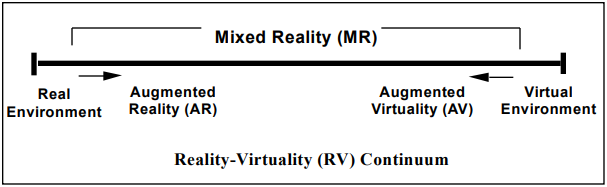
\includegraphics[width=0.75\textwidth]{figures/mixed_reality.png}
			\caption{Example picture that was taken from an external source \takenFrom{asc_notes}.}
			\label{fig:mixed_reality}
		\end{figure}
		\todo{Untertitel bearbeiten}
		
		- Head Mounted Display
		- Mischung von Realität und virtuellen Elementen
		- AR lebt von der realen Welt und somit von freiem Bewegen
		-> nicht an Pc gebunden
		--> weniger Leistung
		--> kein Handtracking
% !TeX root = ../main.tex

\chapter{Verwandte Arbeiten}\label{chapter:background}
	
	%In this chapter, \dots

	%\section{Math} \label{sec:full_grids}
	
		%Math:
		%\begin{align}
			%\Phi(x) = \max(1 - \abs{x}, 0)
		%\end{align}
		
	 %\subsection{Example Figure} \label{sec:back_nodal_hierarchical_basis}
		
		%\begin{figure}[htbp]
			%\centering
			%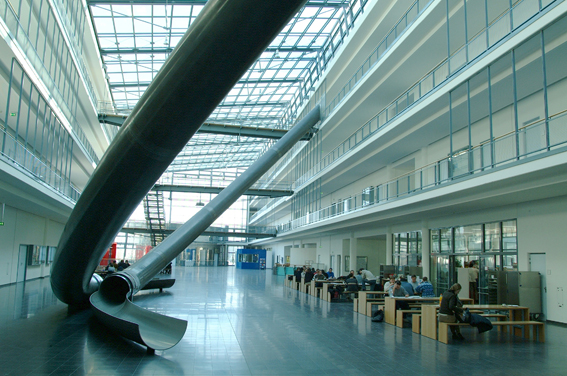
\includegraphics[width=0.5\textwidth]{figures/tum.jpg}
			%\caption{Example picture that was taken from an external source \takenFrom{asc_notes}.}
			%\label{fig:nodalBasis}
		%\end{figure}
		
		%References on figures work like this: blblablabla (see \refFigure{fig:nodalBasis}). If you used external knowledge for a paragraph, use the cite command at the very end of a sentence but right before the full stop \cite{ba_molzer}.
		
		%If you use an $l$ for math symbols, use $\ell$ instead for better readability.
		
	Vor dem Behandeln eines Problems ist es wichtig sich ebenso darüber zu informieren, was in diesem Bereich bereits in anderen Arbeiten behandelt wurde und welche Ergebnisse dabei erzielt wurden. Für diese Arbeit sind beispielsweise die Forschungen im Bereich der Platzierung von Benutzeroberflächen in 2D- und 3D-Anwendungen relevant, ebenso wie das Themenfeld der Priorisierung von anzuzeigenden Informationen.
	Während Forschungen im Bereich der Positionierung und des Designs von Nutzeroberflächen in Desktop-Anwendungen bereits auf jahrelange Erfahrung zurückblicken können, steht man dort bei HMD-Anwendungen noch relativ am Anfang.
	Auch bei dem Thema plattformübergreifender Programme in der erweiterten Realität gibt es schon einige Ansätze, wie ein Projekt von der Organisation Mozilla und eine Reihe von VR- und AR-Spielen zeigt \cite{firefox}\cite{crossCB}.
	Bei näherer Betrachtung dieser Programme fällt jedoch auf, dass hierbei nicht das ganze Potential zur Anzeige von Informationen ausgeschöpft wurde. 
		
	\section{Priorisieren von Benutzeroberflächen}\label{chapter:prio}
		Das Umstrukturieren von Menüs ist nicht trivial, denn jede Veränderung in der Benutzeroberfläche kann das Nutzererlebnis drastisch verändern, falls der Nutzer dadurch irritiert wird. Dies ist sowohl in zweidimensionalen Programmen der Fall, wie auch in der virtuellen dreidimensionalen Welt.
		Mit diesem Nutzererlebnis setzt sich seit einigen Jahren der Bereich des UX Designs (User Experience Design) auseinander.
		Ein wichtiger Aspekt davon ist es, dem Nutzer sowohl nicht zu viel als auch nicht zu wenig Informationen auf einmal zu geben. Dies könnte sonst zu einer Überfordert führen, beziehungsweise durch mangelnde Daten die Nutzung erschweren.
		Es gibt für dieses Problem jedoch keine klare Lösung, da es sich dabei um ein subjektives Erlebnis handelt.
		Um aber das Risiko einer Verschlechterung des Nutzungserlebnisses gering zu halten, hilft es die vorhandenen Informationen zu priorisieren und abhängig davon zu entscheiden, wann und wie diese dem Nutzer angezeigt werden. Dazu verwendet man normalerweise Untermenüs, Tabs oder Ähnliches.\cite{UXNatoli}
		
		
		Dies lässt bereits eine klare Priorisierung erkennen.
		Ausgehend von der Darstellung eines Elements der Benutzeroberfläche in einem Desktop-Programm, kann dessen Wichtigkeit in vier grobe Kategorien einteilt werden.
		
		In die Kategorie mit der höchsten Priorität fallen jene Objekte, die immer angezeigt werden, egal wie das Programmfenster verformt wird. Notfalls wird dafür sogar die Skalierung eingeschränkt. Typische Beispiele für diese Kategorie sind die \term{Speichern}- und die \term{Programm Schließen}-Schaltflächen.
		
		Etwas weniger wichtige Informationen werden zwar auch immer versucht anzuzeigen, aber falls der Platz dafür nicht ausreichen sollte, werden sie etwa in ein temporäres Untermenü verschoben oder auf andere Weise minimiert. Sobald wieder genug Platz vorhanden ist, tauchen sie erneut an der gewohnten Stelle auf. Dazu zählen unter anderem Hilfsfunktionen, wie das \term{Einfügen} oder \term{Ausschneiden} in Texteditoren.
		
		Untermenüs beherbergen die nächst tiefere Kategorie. Deren Inhalt kann manuell angezeigt werden, aber ist sonst nie sichtbar. Es handelt sich meist um sekundäre Funktionen, die nur gelegentlich benötigt werden.
		
		Die unwichtigsten Elemente befinden sich in Menüs innerhalb von Untermenüs und sind somit nur durch mehrere Interaktionen auffindbar. Im Normalfall sind dieses Einstellungen, welche nur selten verwendet werden.
		%- Elemente immer angezeigt (typisch Speichern und Exit)
		%- Elemente können versteckt werden (Funktionen Einfügen/Ausschneiden)
		%- Elemente in Untermenü (dropdown)
		%- elemente in Unteruntermenüs (Funktionen, die selten verwendet werden z.B Einstellungen)
		
		Tabs erzeugen jedoch Ausnahmen bei dieser Einordnung. Sie stellen sozusagen verschiedene Kontexte dar, in welchen die Prioritäten anders verteilt sein können. So existieren möglicherweise in einem Kontext bestimmte Informationen nicht, aber in einem anderen werden sie durchgehend angezeigt. Aus diesem Grund wird zwischen kontextabhängigen und -unabhängigen Elementen unterschieden.
		
		%- UX
		%- Prioritätsgruppen
		%- Umsetzung in 2D
		
	\section{Positionierung in 2D-Anwendungen}
		Das verbreitetste Konzept bei der Erstellung von Nutzeroberflächen ist das WIMP-Konzept. Die Abkürzung steht für \term{Windows}, \term{Icons}, \term{Menus} und \term{Pointers}. 
		Damit deutet sie bereits darauf hin, wie man sich die Umsetzung dieses Konzepts vorstellen kann. Programme werden bei dieser nämlich als Fenster dargestellt. Diese können weitere Fenster enthalten oder auch Menüs, in welchen Inhalte angeordnet sind. Um Funktionen möglichst kompakt anzeigen zu können, werden diese teilweise in Form von einem Bild oder Zeichen, einem sogenannten \term{Icon} dargestellt.
		Als Anker zum Positionieren des Fensterinhalts dienen jeweils die Eckpunkte des Fensters. Die einzelnen Elemente werden in den Fenstern also immer relativ zu mindestens einer Ecke des jeweiligen Fensters platziert. Dadurch kann der Inhalt eines Programmfensters bei dessen Verschiebung oder Skalierung mitbeweget werden. Damit ein Objekt sich zudem mit dem enthaltenden Bildausschnitt vergrößert, verkleinert oder darin zentriert bleibt, muss es hingegen an zwei oder mehr Ecken gebunden werden. Dies wird in der \refFigure{fig:unity} aus der Spiel-Engine Unity am rechten und unteren Rand dargestellt.
		%Damit sich Programmfenster beliebig vergrößern lassen, auch unabhängig von den ursprünglichen Seitenlängenverhältnissen, ohne dass der Inhalt an einer Seite abrupt abgeschnitten wird, muss 
		%- Windows Icons Menus Pointers
		
		%- Menüs / Fenster
		%Menüs geben eine Auswahl von Funktionen in Form von ...
		%- Bildschirmränder
		
		
	\section{Positionierung in 3D-Anwendungen}\label{chapter:3dPos}
		
		In Programmen, die eine dreidimensionale virtuelle Welt anzeigen (im Folgenden \term{3D-Programm} genannt), wird eine spezielle Form der graphischen Benutzeroberfläche verwendet. Diese liegt nicht in einer zweidimensionalen Ebene vor der Kamera, sondern befindet sich im dreidimensionalen Raum. Dies ermöglicht auch nicht-planare Formen, was dieser Abwandlung den Namen \term{3D User Interface} gab.
		
		Diese dreidimensionalen Elemente werden in 3D-Programmen für Desktop-Geräte gewöhnlich an festen Orten angebracht und bewegt sich gegebenenfalls an einem Objekt der Umgebung mit. Dies wird auch als diegetische Benutzeroberfläche bezeichnet, da sie tatsächlich Teil der virtuellen Welt ist.
		
		In VR- und AR-Anwendungen steht teilweise zusätzlich die Option zur Verfügung, einen virtuellen Gegenstand oder eine Anzeige an den Handpositionen des Nutzers zu befestigen, oder ihn mit der Nutzeroberfläche auf andere Arten räumlich zu umgeben. Dies bietet dem Benutzer eine natürliche Art der Interaktion. Um etwas auszuwählen könnte er einfach auf das gewünschte Element zugehen und nach ihm die Hand ausstrecken. Denkbar ist eine solche Umsetzung unter anderem in Form eines Zylinders, wie in \refFigure{fig:cylinder_mapping} dargestellt.
		
		%- 3D Programm: UI in Welt platziert
		%- Üblich Hände und Kopf oder an statischen Objekten
		In dieser Arbeit wurden als Ankerpunkte für solche Elemente die beiden Handpositionen des Benutzers und die Kopfposition verwendet, da diese Stellen im Fall der Verwendung von Erfassungssystemen durch Controller, das HMD oder die reale Hand gegeben sind.
		
		\begin{figure}[htbp]
			\centering
			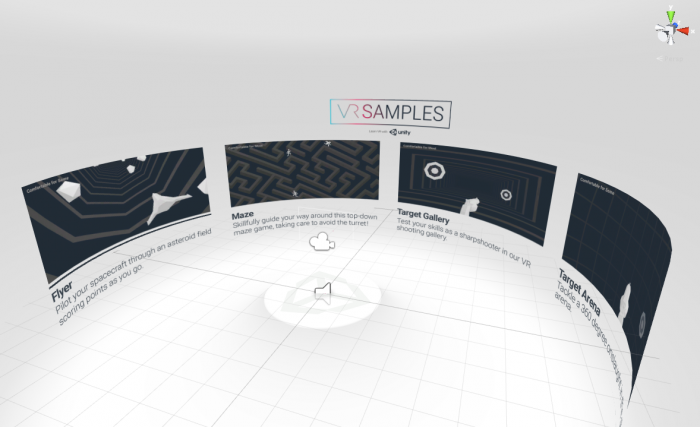
\includegraphics[width=0.75\textwidth]{figures/cylinder_mapping.png}
			\caption{Example picture that was taken from an external source \takenFrom{unityCurved}.}
			\label{fig:cylinder_mapping}
		\end{figure}
% !TeX root = ../main.tex

\chapter{Problemdiskussion}\label{chapter:dimensionwise_refinement}

	%References for chapters work like this. blblbla see \refChapter{chapter:background}.
			
	%\section{Program Structure}
	
		%For program code, use the following structure:
		
		%\begin{figure}[htbp]
			%\centering
			%\begin{tabular}{c}
			%\begin{lstlisting}[language=python]
			%	# enter your code here (# marks a comment in python)
			%	def (stuff as stuff):
			%		x = 1
			%	\end{lstlisting}
			%\end{tabular}
			%\caption{Caption Example}
			%\label{fig:code_integrator}
		%\end{figure}
		
	\section{Problembeschreibung}
		Da es viele verschiedene Umsetzungen der virtuellen und erweiterten Realität gibt, steht man als Entwickler eines Mixed-Reality Programms über Kurz oder Lang vor einigen Hindernissen. Eines davon ist die Platzierung der Benutzeroberfläche, da hierbei im Gegensatz zu gewöhnlichen Desktop-Anwendungen keine Bildschirmränder oder vergleichbare Begrenzungen existieren.
		Zudem gibt es keine konkrete Vorgabe wie die Benutzeroberfläche in der dreidimensionalen Welt platziert werden sollte. \todo{Weiter}
		Häufige Umsetzung - Hände oder Zylinder
		\todo{Bis hier überprüfen}
		Besondere Schwierigkeiten entstehen aber noch zusätzlich, wenn man das Programm auf verschiedenen Geräten nutzen möchte. So werden zum Beispiel bei vielen Varianten der erweiterten Realität die Handpositionen nie oder zumindest nicht kontinuierlich verfolgt und ermöglichen somit kein konstantes Anzeigen von virtuellen Elementen an diesen Stellen. Sie können daher schlecht als Ankerpositionen für die Benutzeroberfläche verwendet werden.
		Andere Geräte stellen durch die Positionserfassung der Controller und der VR- oder AR-Brille die Kopf- und Handpositionen zu jeder Zeit zur Verfügung. Das Wegfallen von Controllern durch niedrigen Akkustand oder andere Umstände erzeugt dabei allerdings ein ähnliches Problem wie bei den Varianten ohne solche Controller.
		Da die Positionierung der Benutzeroberfläche an den Handpositionen deutlich mehr Möglichkeiten eröffnet \todo{Beweis?}, sollten diese auch genutzt werden, solange sie vorhanden sind. Für den Fall ihrer Abwesenheit ist es dann allerdings nötig eine Rückfallmöglichkeit bereitzustellen, damit keine Elemente der Benutzeroberfläche verloren gehen und mit ihnen deren Funktion und Information. Diese Verluste könnten sonst eine produktive Nutzung erschweren oder sie sogar gänzlich verhindern.
		
	\section{Ansatz}
		Um die Verwendung von allen Elementen der Benutzeroberfläche auch beim Verlust einer oder mehrerer möglicher Ankerpositionen zu gewährleisten, wurden in dieser Arbeit mehrere Möglichkeiten erarbeitet, um eine Umverteilung der enthaltenen Informationen von einem nicht verwendeten Anker auf einen oder mehrere aktive Anker durchführen zu können.
		Dafür wird betrachtet wie wichtig die einzelnen Inhalte sind, welche aktiven Ankerpositionen zur Verfügung stehen und was für eine Rückfallart bei der Verschiebung verwendet werden soll. Letztere entscheidet darüber wie der Rückfall aufgefangen wird.
		Die Neuplatzierung der umverteilten Bausteine übernimmt jeweils der neue Anker.
		\todo{fortsetzen?}
		
		\subsection{Umsetzung der Prioritätsstufen}
			Um herauszufinden wie wichtig ein Element ungefähr ist, werden erst klare Klassen benötigt, welche unterschiedliche Prioritäten darstellen. Diese entscheiden darüber wie und wo eine Information dargestellt wird und ebenso wohin sie, im Falle des Verlusts des zugehörigen Ankers, verschoben wird.
			Als Vorbild für das in dieser Arbeit verwendete Modell dient das Konzept S.H.I.T., welches von ...
			Es teilt Informationen in vier \todo{?} Kategorien ein:
			- Should
			- 
			-
			- Treasure
			
			%- vorbild S.H.I.T.
			%- wichtig für Verarbeitung bei Fallback
			
			- High/Medium/Low/None
			Zudem wurde es abhängig vom aktuellen Kontext und dem Typ der Ankerposition gemacht.
			%- Kontextabhängigkeit
			
			Hand:
			-Hoch Immer angezeigt
			-Medium Immer angezeigt
			-Low Zuschaltbar
			-None Zuschaltbar 
			
			Kopf:
			-Hoch: immer angezeigt, immer sichtbar
			-Medium immer angezeigt
			-Low Zuschaltbar
			-None Fällt weg
			
		\subsection{Rückfallarten}
			Beim Umverteilen der Ankerinhalte ... irgendwas mit Balance zwischen individueller Platzierung und automatisiert in Blöcken sowie Nutzbarkeit\todo{Formulieren}
			%- Über ID
			Eine Variante, welche manuelles Platzieren ermöglicht, ist die Verschiebung über eine Identifikationsnummer. Dabei werden, gegebenenfalls veränderte, Kopien des zu verschiebenden Inhalts bereits vorher auf den Rückfall-Ankern platziert. Beim Wegfallen des Ankers wird dann lediglich auf diesen Ankern nach einem Element mit der gleichen Identifikationsnummer gesucht und dieses aktiviert. - Nachteile - Vorteile \todo{Formulieren}
			
			
			%- Über Container
			Eine andere Möglichkeit, welche ein automatisiertes geordnetes Platzieren umsetzt, benötigt eine Art Container für Inhalte. Ein Beispiel für einen solchen Container sind die Anker selbst, da sie ebenso Elemente enthalten. Allerdings ordnen diese von sich aus keine neuen Informationen auf bestimmte Weise neben den Bestehenden an, sondern übergeben diese Aufgabe an andere Container, welche in ihnen enthalten sind. Die Art und Weise wie ein Container neue Inhalte handhabt muss manuell festgelegt werden und wird dann zur Laufzeit automatisiert ausgeführt. - Nachteile - Vorteile \todo{Formulieren}
			
			
			%- Innerhalb eines Containers
			Zuletzt gibt es noch eine Art der Verschiebung, bei der die betroffenen Elemente innerhalb ihres Behälters bleiben und dieser dann mitsamt seinem Inhalt als ein Objekt verschoben wird. Dabei muss der Zielanker auf eine, in \todo{Kapitelverweis}beschriebene, Weise erweitert werden, da dem Anker die genaue Lage des Inhalts nicht bekannt ist. - Nachteile - Vorteile \todo{Formulieren}
			%- Wichtigkeit entscheidet über nutzbare Anker
			Bei allen Varianten wird geprüft ob die Priorität des verschobenen Objekts höher oder gleich wie die Mindestpriorität des Zielankers ist, um jederzeit möglichst nur die benötigte Information anzuzeigen und unwichtige Inhalte gegebenenfalls zu verbergen. Falls die Priorität nicht zu dem Anker passen sollte, wird das Verfahren auf einem anderen Anker weitergeführt, solange noch ein weiterer zur Verfügung steht.
			
		\subsection{Erweiterung}
			\todo{Überarbeiten und Kapitel darüber referenzieren}
			Wie bereits in ... erwähnt, kann es vorkommen, dass ein Anker durch das Verschieben von Informationen eines anderen Ankers gegebenenfalls erweitert werden muss, um die zusätzlichen Elemente platzieren zu können.
			Zum Erweitern eines Ankers wurden hierbei folgende zwei Varianten erarbeitet.
			
			%- Directional
			Bei der ersten Art wird der Bereich, in dem der Inhalt platziert werden kann, in eine vorgegebene Richtung erweitert. Daraufhin werden der neue und der alte Inhalt darin untereinander beziehungsweise nebeneinander platziert.
			
			
			- Switch
			
			Die andere Variante nutzt das ... Umschalten
			Somit wird nicht mehr Platz eingenommen.
			Allerdings kann man dadurch die verschiedenen Informationen nicht alle gleichzeitig sehen.
			
			
			
		%\subsection{TODO}
			\todo{Bereich Ankertype oder Ankerstyle möglich}
			
	\section{Umsetzung}
		Um diesen Ansatz umzusetzen wurden die Klassen \term{UIAnchor}, \term{AnchoredUI}, \linebreak\term{AnchorManager} und das Interface \term{UIContainer} in der Programmiersprache C\# erstellt. \todo{Mehr}
			
		\subsection{UIAnchor}
			Die Klasse \term{UIAnchor} stellt einen Anker für Bestandteile der Benutzeroberfläche dar. Sie beinhaltet unter anderem die Attribute \term{style} und \term{type}, welche angeben, inwiefern der Inhalt des Ankers manipuliert werden soll. \todo{Wie wird er manipuliert?}
			
			Außerdem hat er noch vier Attribute, welche seine Bindung zum zugehörigen Ankerobjekt darstellen. Eins gibt die relative Position des Ankermittelpunkts zur Mitte des Ankerobjekts an. Ein weiteres steht für die relative Rotation zu diesem Objekt. Die anderen beiden Variablen legen fest, ob und wie sich der Anker mit dem Ankerobjekt rotiert. \todo{Ankerobjekt in umgebungsabhängig definieren}
			%- Rotation/Translation zu Ankerposition
			- Erweiterungsart
			- minprio
			%- statictoObj
			%- rotates
			%- stellt Anker dar
			Zudem hat die Klasse eine optionale Referenz auf eine weitere Ankerinstanz, welche im Nachfolgenden \term{Kindanker} genannt wird. Diese sollte im Normalfall eine niedrigere Mindestpriorität besitzen und vom gleichen Typ sein, denn sie dient als weitere Möglichkeit für die Platzierung von Inhalten, falls diese in dem Anker mit höherer Mindestpriorität keinen Platz finden. Außerdem wird durch die Kindanker das Platzieren mehrerer Anker an einem einzelnen Objekt ermöglicht. - Deaktivierung mit Vateranker
			%- gibt Anweisungen an Kinderanker weiter
			%- Manipuliert Elemente abhängig von Ankertyp
			- Setzt Fallback um
			Beim Nichtvorhandensein des Objekts, an der ein Anker platziert werden sollte, sucht dieser über die statische Klasse \term{AnchorManager} nach einem alternativen Ort, um seine Informationen weiterhin anzeigen zu können.
			Falls kein Anker dafür gefunden wurde, wird die Information verworfen und eine Warnmeldung angezeigt. Ansonsten wird versucht diesem den Inhalt zu übergeben. Der Zielanker berechnet dann mittels dessen Priorität, ob er die Informationen bei sich platziert oder sie an einen Kindanker weiterleitet.
			
			- Cylinder (Beispiel Bild bereits verwendet - Referenz)
			- Rectangle 
			- Umsetzungen abhängig von Prio und Position
			- Vorbild Rectangle Hololens
			\begin{figure}[htbp]
				\centering
				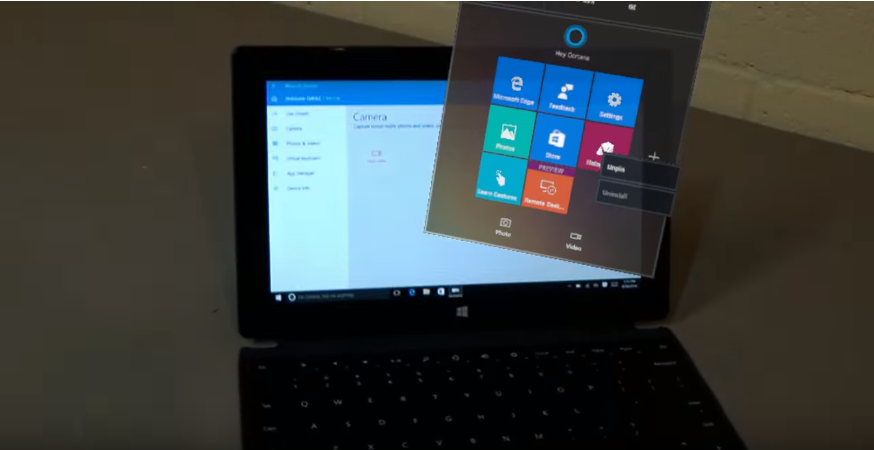
\includegraphics[width=0.75\textwidth]{figures/HololensMain.png}
				\caption{Menü der Hololens \takenFrom{hololens}.}
				\label{fig:hololensMain}
			\end{figure}
			- Cylinder Abwandlung von Planetarium und Ähnlichem
		
		\subsection{UIContainer}
			Dieses Interface dient als Vorlage für Behälter von Instanzen der Klasse \term{AnchoredUI}. \linebreak Diese Container enthalten eine Logik zum systematischen Platzieren von neuen\linebreak Elementen innerhalb des bereits vorhandenen Inhalts.\todo{Mehr}
			%- enthält Elemente
			%- ermöglicht strukturierte Platzierung von dynamischem Inhalt
		
		\subsection{AnchoredUI}
			Die einzelnen Elemente der Benutzeroberfläche werden durch Instanzen dieser Klasse repräsentiert. Sie beinhaltet Informationen für die Umsetzung der ...
			\todo{Mehr}
			%- Stellt Element dar
			%- Beinhaltet Informationen für die Fallback Umsetzung
		
		\subsection{AnchorManager}
			- Regelt das Wegfallen von Ankern
			- Weist FBAnker zu
			
	\section{Evaluierung}
		%- Studie
		%- 13 Teilnehmer
		Um die beschriebene Umsetzung zu evaluieren wurde eine Nutzerstudie durchgeführt, an der dreizehn Freiwillige im Alter zwischen 16 und 26 Jahren teilnahmen. Dieses Kapitel beschreibt deren Aufbau und Ablauf.
	
		\subsection{Studienablauf}
			%- 4 Szenarien
			In der Studie mussten die Probanden in vier verschiedenen Szenarien jeweils eine Reihe von Aufgaben durchführen. Die Reihenfolge der vier Abschnitte wurde dabei jedes Mal variiert und war für jeden Teilnehmer unterschiedlich, um einen Einfluss der Bearbeitungsreihenfolge auf das Gesamtergebnis möglichst gering zu halten. Die Aufgabenstellung blieb in allen Szenarien die Gleiche.
			
			
						
			Zu Anfang sollten die Tester ein paar einleitende Fragen beantworten, dann führten sie die Aufgaben ein erstes Mal in einem der Szenarien durch und beantworteten danach Fragen zu diesem Testfall und einzelnen Elementen darin. 
			Dies beinhaltete zwei Fragen nach der gefühlten Schwierigkeit der Aufgabe innerhalb des Testfalls. Einmal sollten sie angeben ob sie gefühlt viel Zeit für die Aufgabe gebraucht haben, beim zweiten Mal mussten sie deren Schwierigkeit auf einer Skala von eins bis fünf bewerten, wobei eins für sehr leicht und fünf für sehr schwierig steht. Zusätzlich sollten sie angeben, ob sie die Positionierung der Benutzeroberfläche übersichtlich oder willkürlich fanden.
			
			
			Danach folgten jeweils drei Fragen zu sieben Elementen der Benutzeroberfläche aus der Testszene. Bei diesen konnten sie jeweils aus einer gegebenen Liste auswählen, ob und warum sie nach dem Element suchen mussten, es anstrengen anzusehen fanden oder es störend fanden. Eine nicht gelistete Antwort konnte ebenfalls angegeben werden.
			%- störend - anstrengend anzusehen - nicht findbar
			%- Aufzählung der Fragen
			
			Die zu bewertenden Elemente wurden so ausgewählt, dass jeweils mindestens zwei Beispiele aus den Prioritätsklassen \term{high}, \term{medium}, \term{low} und zwei kontextabhängige Exemplare bewertet wurden.
			%- Wie wurden zu bewertende Elemente ausgewählt?
			Die Auswahl dieser Elemente war ebenfalls in jedem Szenario gleich.
			
			Dies wurde viermal wiederholt. Zum Abschluss sollten sie noch angeben, wie schwierig sie die Aufgabenstellung und die Steuerung unabhängig von den Szenarien fanden und als wie wichtig sie die ausgewählten Elemente auf einer Skala von eins bis fünf einordnen würden. Die genauen Definitionen der verschiedenen Stufen wird in \refChapter{chapter:resultsPrio} beschrieben.
		
		\subsection{Szenario-Beschreibung}\label{chapter:szenario}
			In jedem der Testfälle hatten die Tester die Aufgabe mit einem offen sichtbaren Gegenstand zu interagieren. Dazu musste der \term{Cursor} auf diesen ausgerichtet werden. Der \term{Cursor} ist in der Mitte des Sichtfeldes platziert und bewegt sich beim Drehen und Neigen des Kopfes mit. Man wählt also im Groben ein Objekt aus indem man darauf schaut.
			Nach dem Interagieren mit dem Gegenstand öffnet sich ein verborgenes Menü. Dieses heißt im Folgenden \term{Handelsfenster}. Es beinhaltet zwölf Elemente mit je einem farbigen Würfel und einer Preisangabe, welche alle ausgewählt werden können.
			
			Als nächstes sollten die Tester herausfinden, wie viel Geld ihnen zur Verfügung steht und dann einen Würfel auswählen, dessen Preis die verfügbare Geldmenge nicht überschreitet. Diese Menge wird im Infofeld \term{Vermögen} angezeigt, welches nur bei geöffnetem Handelsfenster verfügbar ist.
			Daraufhin wird der ausgewählte Würfel gekauft und in das Feld \term{Ausgewähltes Objekt} verschoben, welches zu jeder Zeit angezeigt wird. Es informiert darüber, ob etwas gerade ausgewählt ist und um was es sich dabei handelt.
			
			Die letzten drei Schritte beinhalten das Legen des gekauften Würfels in eines der \term{Inventar}-Felder, das erneute Auswählen des Würfels und das Ablegen in ein Feld der \term{Ausrüstung}. Sowohl das \term{Inventar} als auch die \term{Ausrüstung} können manuell ein- und ausgeblendet werden. Wie dies funktioniert und wie die beiden Elemente erkannt werden können wurde den Teilnehmern vor dem Ausführen der Aufgabe erklärt.
			Danach gilt die Aufgabe als abgeschlossen.
			
			Die vier Szenarien unterscheiden sich nur in der Platzierung der genannten Elemente der Nutzeroberfläche.
			\todo{Beschreiben}
			%- Szenenbeschreibung
			%- verwendete UI Elemente
			- Unterschiedliche Fälle
		
% !TeX root = ../main.tex

\chapter{Ergebnisse}\label{chapter:results}

	\section{Prioritäten}
	
		- Tabelle zu Prioritätsbewertung
	
	\section{Bewertung der Szenarien}
% !TeX root = ../main.tex

\chapter{Fazit}\label{chapter:conclusion}

	Im Nachfolgenden werden die wichtigsten Ergebnisse dieser Arbeit kurz zusammengefasst und es wird ein Ausblick darüber gegeben, was man in Zukunft potentiell an dem Konzept verbessern könnte, beziehungsweise inwiefern man es erweitern kann. Dies beinhaltet ebenso die Grenzen und Schwächen dieser Arbeit.

	\section{Zusammenfassung}
	
		Die in dieser Arbeit entwickelten Konzepte
		- Relativ wenige Tester
		- Steuerung war für einige Nutzer nicht intuitiv aber mit Übung ging es
		- Umsetzung fanden die Tester im Groben gut?
		
		- mitbewegende DauerUI wurde negativ bewertet, zu groß, zu nah
		- Schwierigkeiten mit verborgenen Elementen
	
	\section{Ausblick}
		
		In der Zukunft wäre eine umfangreichere Studie nützlich, um die Wirkung einzelner Elemente auf die Nutzer besser zu erfassen und ein genaueres Abbild der durchschnittlichen Nutzermeinung zu erhalten. Dazu ist es nötig weitere Altersgruppen miteinzubeziehen, wie zum Beispiel mehr Tester, welche zwischen 13 und 18 oder 25 und 40 Jahren alt sind. Die bisherige Studie umfasst nämlich lediglich den Altersbereich 16 bis 26. Außerdem muss die Anzahl der Teilnehmer erhöht werden.
		
		
		Des weiteren kann die Umsetzung einiger Elemente des, über diese Arbeit erstellten, Programms verbessert werden. So wäre es zum Beispiel sinnvoll, die einzelnen zweidimensionalen Objekte eines Zylinderankers so zu verformen, dass sie tatsächlich auf der Oberfläche des Zylinders angezeigt werden und somit selbst unterschiedlich große Elemente nahtlos nebeneinander platziert werden können. Bisher sind sie noch planar und nur ihr Mittelpunkt  liegt auf dem Zylinder, was besonders bei großen Elementen dazu führt, dass deren seitliche Kanten deutlich weiter vom Zylindermittelpunkt und somit vom Standpunkt des Nutzers entfernt sind.
		Denkbar wäre es außerdem das Prinzip des Zylinders ebenso auf eine Kugel umzuformen
		\todo{Graphisch darstellen}
		
		
		Zudem fehlen bisher noch alternative Implementierungen von Containern neben den Ankern, welche eine sinnvolle und einfache Umlagerung von Bausteinen zwischen zwei verschiedenen Ankern ermöglichen. Möglich wären auch Container für andere Container.
				
		
		Ein weiteres wichtiges Thema, welches in dieser Arbeit nicht behandelt wurde, aber in diesem Bereich in Zukunft eine große Rolle spielen wird, ist die Begrenzung des Informationsumfangs an einem einzelnen Anker. Dies ist nämlich ein wichtiger Punkt im Hinblick auf das Nutzererlebnis. Zu viel Information kann den Nutzer überfordern beziehungsweise stören, wie man bei der Auswertung der Umsetzung mit nur der linken Hand in \refChapter{chapter:resultsSzen} sieht.
		
		
		Zur Erleichterung der Interaktion wäre die Entwicklung verschiedener Interaktionsformen für die einzelnen Szenarien praktisch. Die in dieser Arbeit verwendete Form war nämlich nicht sonderlich intuitiv und nutzt das Potential der Controller nicht.
		
		
		Die Probleme des umschaltbaren Menüs könnte man durch eine klare Beschriftung eventuell verbessern. Das Anbringen eines kleinen Hinweises, welcher am Rand des Sichtfelds auftaucht, könnte das Finden verborgener Elemente ebenfalls weiter vereinfachen.
	
		
		%-Verformen der UI
		%-Containerimplementierung
		%-Wie viel UI?
\nocite{milgram}

\appendix{}

\microtypesetup{protrusion=false}
\listoffigures{}
\listoftables{}
\microtypesetup{protrusion=true}
\printglossaries
\printbibliography{}
% !TeX root = ../main.tex

\chapter{Appendix}\label{chapter:appendix}

	
% !TeX root = ../main.tex

\chapter{Fragebogen: Platzierung von Benutzeroberflächen in VR - Einleitung}\label{chapter:fragen}
	\begin{figure}[htbp]
		\centering
		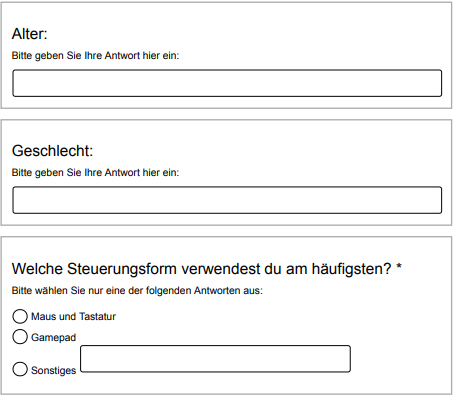
\includegraphics[width=0.6\textwidth]{Fragen/1Einleitung.png}
	\end{figure}

	\begin{figure}[htbp]
		\centering
		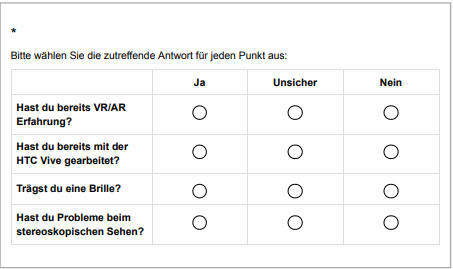
\includegraphics[width=0.6\textwidth]{Fragen/2Einleitung.png}
	\end{figure}
\chapter{Fragebogen: Platzierung von Benutzeroberflächen in VR - Szenario}\label{chapter:fragen2}
	\begin{figure}[htbp]
		\centering
		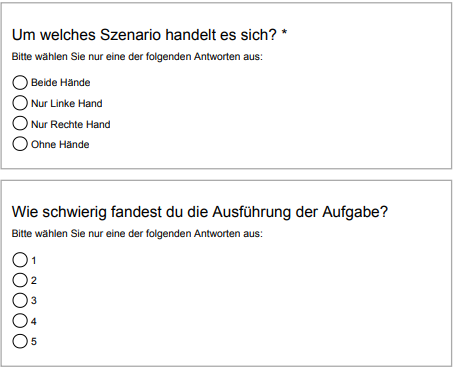
\includegraphics[width=0.75\textwidth]{Fragen/1Szenario.png}
	\end{figure}

	\begin{figure}[htbp]
		\centering
		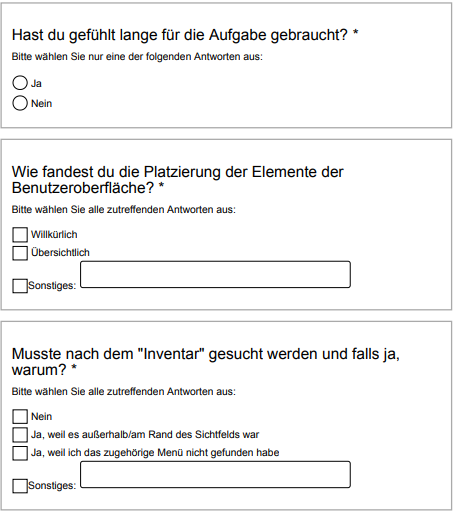
\includegraphics[width=0.75\textwidth]{Fragen/2Szenario.png}
	\end{figure}

	\begin{figure}[htbp]
		\centering
		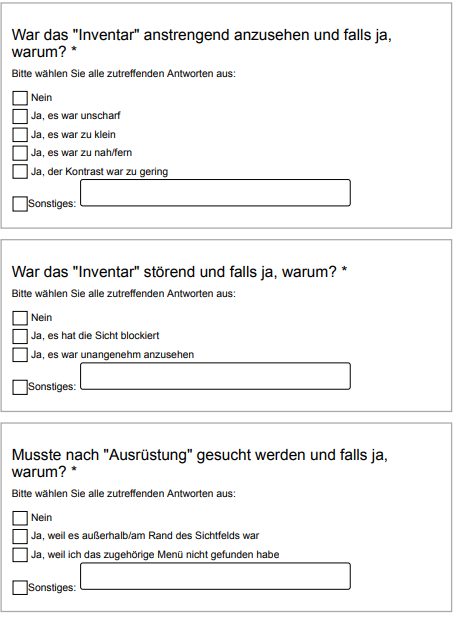
\includegraphics[width=0.75\textwidth]{Fragen/3Szenario.png}
	\end{figure}

	\begin{figure}[htbp]
		\centering
		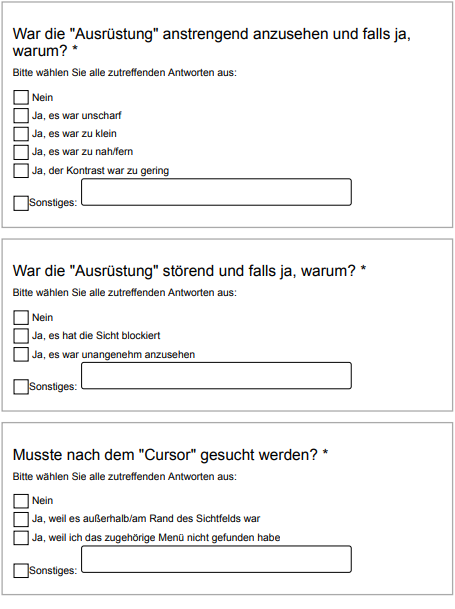
\includegraphics[width=0.75\textwidth]{Fragen/4Szenario.png}
	\end{figure}

	\begin{figure}[htbp]
		\centering
		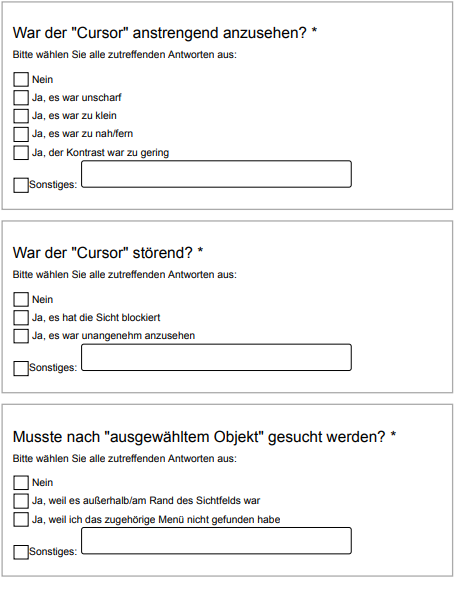
\includegraphics[width=0.75\textwidth]{Fragen/5Szenario.png}
	\end{figure}

	\begin{figure}[htbp]
		\centering
		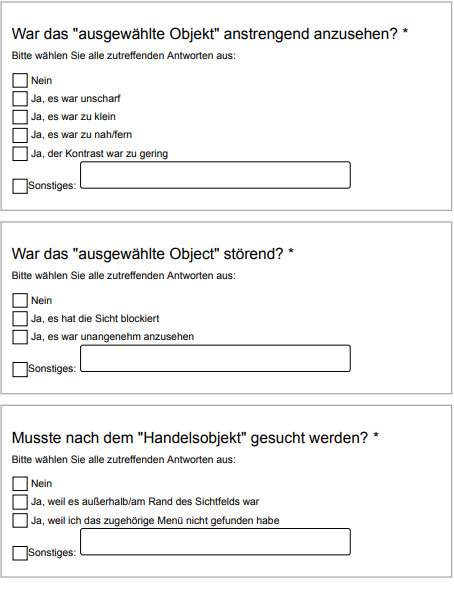
\includegraphics[width=0.75\textwidth]{Fragen/6Szenario.png}
	\end{figure}

	\begin{figure}[htbp]
		\centering
		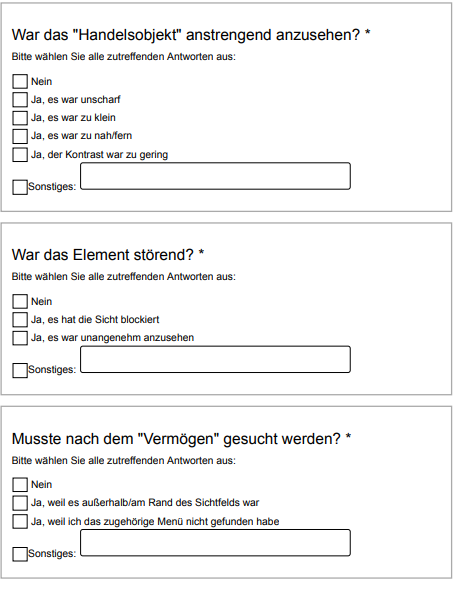
\includegraphics[width=0.75\textwidth]{Fragen/7Szenario.png}
	\end{figure}

	\begin{figure}[htbp]
		\centering
		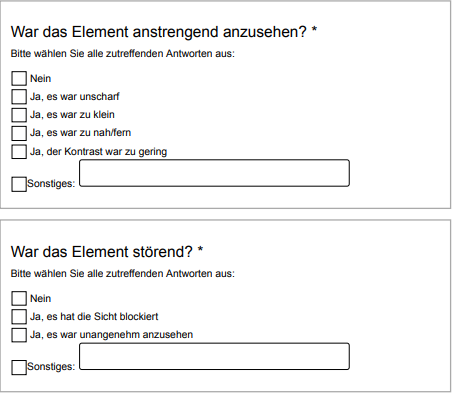
\includegraphics[width=0.75\textwidth]{Fragen/8Szenario.png}
	\end{figure}
% !TeX root = ../main.tex

\chapter{Fragebogen: Platzierung von Benutzeroberflächen in VR - Abschluss}\label{chapter:fragen3}
	\begin{figure}[htbp]
		\centering
		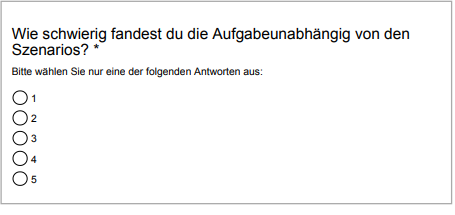
\includegraphics[width=0.7\textwidth]{Fragen/1Ende.png}
	\end{figure}

	\begin{figure}[htbp]
		\centering
		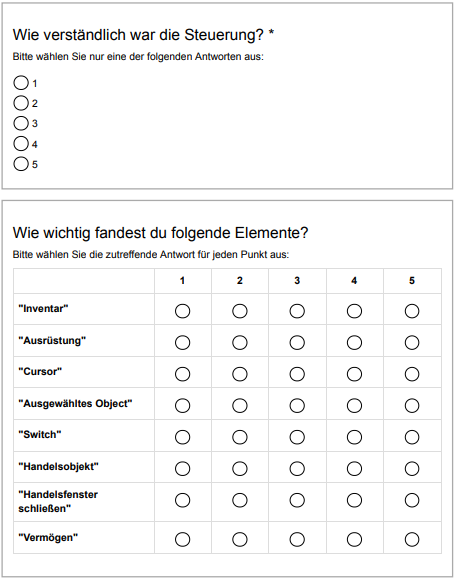
\includegraphics[width=0.7\textwidth]{Fragen/2Ende.png}
	\end{figure}
\end{document}
